\section{Vergleich mit Anforderungen} \label{Anforderungsvergleich}

	Alle Anforderungen werden mit der erarbeiteten Lösung verglichen und auf die in Kapitel \ref{Projektanforderungen} definierten Anforderungen bezogen.  Die Anforderungen werden wie folgt bewertet:
	\begin{table}[H]
		\centering
		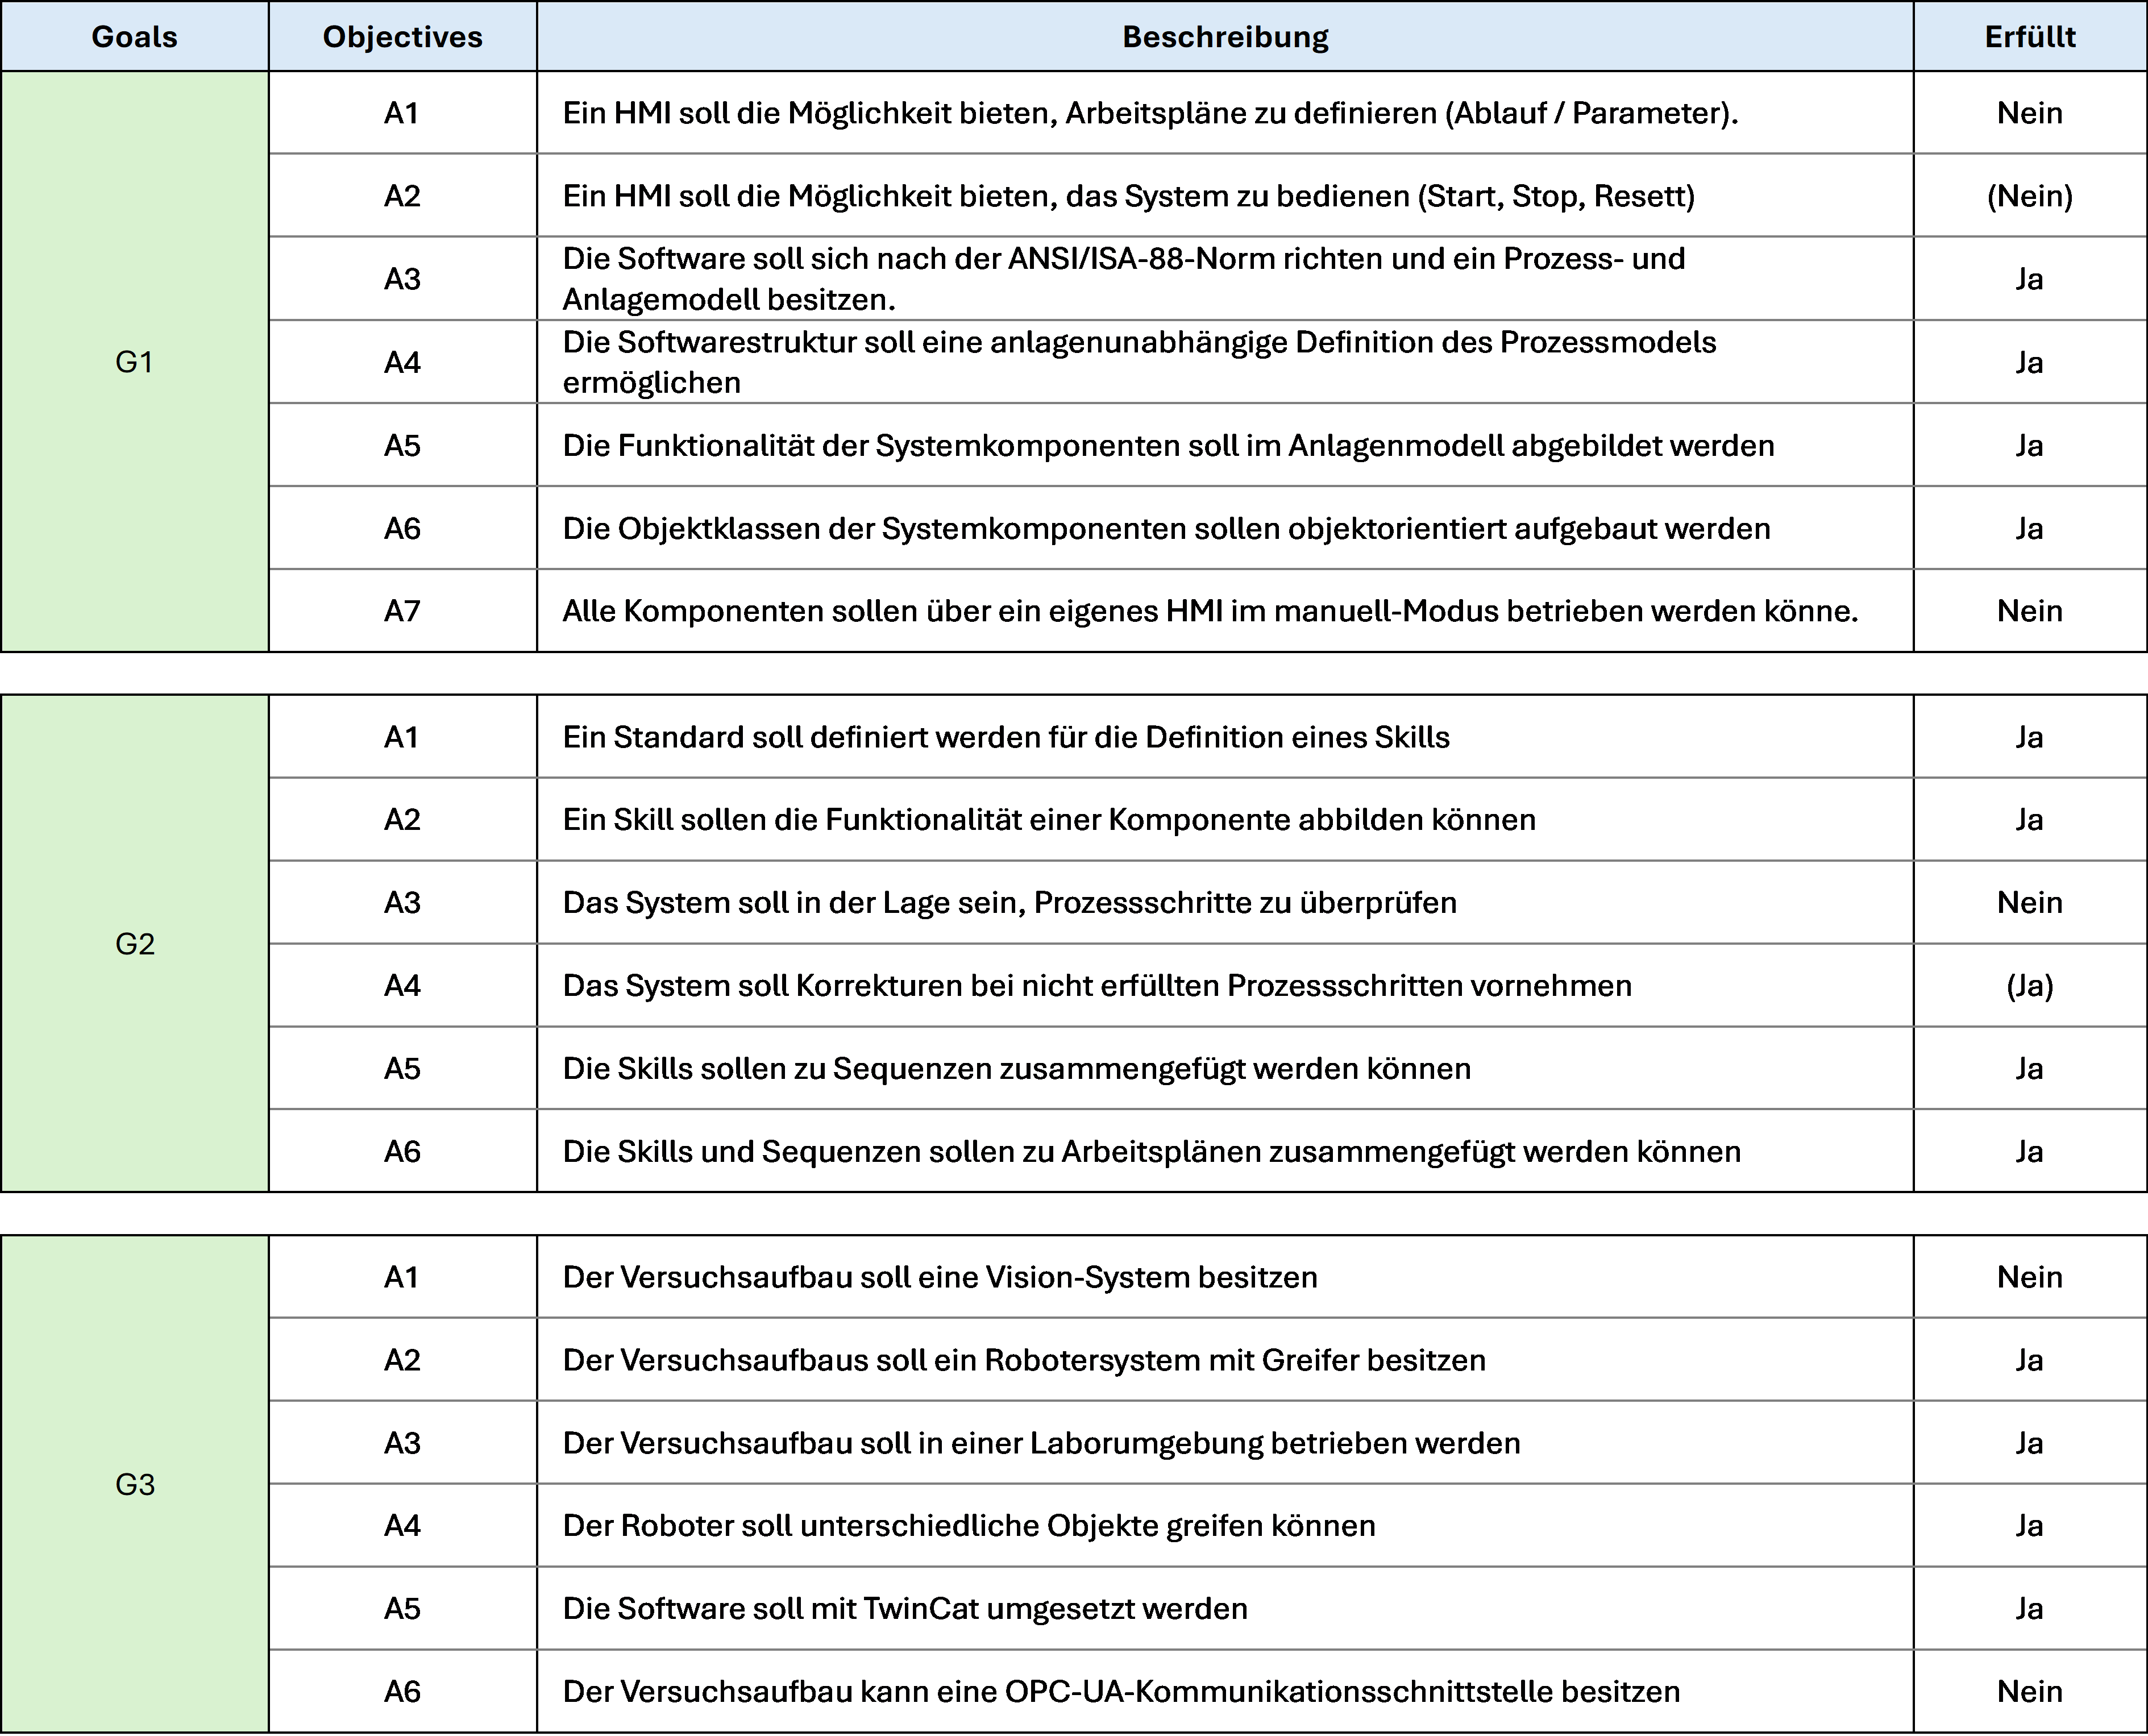
\includegraphics[width=0.9\textwidth]{09_Auswertung/Anforderungsvergleich}
		\captionsetup{justification=centering}
		\caption{Vergleich mit Anforderungen}
		\label{tab:Anforderungsvergleich}
	\end{table}
	
	Viele der Anforderungen wurden mit der erarbeiteten Lösung erfüllt. Dennoch gibt es einige
	Anforderungen, die nicht oder nur teilweise erfüllt wurden:
	
	\begin{tabularx}{\textwidth}{@{}>{}p{4em} X@{}}
		G1 / A1: & 
		Im Moment wurde nur ein sehr einfaches und provisorisches HMI realisiert, damit der allgemeine Ablauf getestet werden kann. Das HMI bietet nicht die Möglichkeit verschiedene Abläufe oder Parameter vorzugeben.
		\\
		G1 / A2: & 
		Das HMI kann grundsätzlich das System starten, stoppen und resetten. Die Umsetzung ist jedoch noch so rudimentär, dass die Anforderung als nicht erfüllt betrachtet wird. Das HMI dient nur dem Testen der Anlage und stellt nicht eine, vom Endbenutzer, anwendbare Lösung dar. 
		\\
		G1 / A7: & 
		Für die verschiedenen Objektklassen wurden noch keine HMI erstellt. 
		\\
		G2 / A3: & 
		Die ursprünglich angedachte Vision, dass sich das System selbständig korrigieren kann, wurde nicht implementiert. Im Verlauf des Projektes wurde festgestellt, dass dieses Feature nur wenig Überschneidungen mit dem definierten Thema hat und grundsätzlich in einem eigenen Projekt umgesetzt werden müsste. Der Fokus dieser Arbeit wurde auf die Software-Struktur gelegt. 
		\\
		G2 / A4: & 
		Das System reagiert zwar nicht selbständig auf nicht erfüllte Prozessschritte, über die Zustände der Skills kann jedoch im Ablauf auf gewisse Situationen reagiert werden (z.B. das Erreichen eines Schwellenwertes).
		\\
		G3 / A1: & 
		Aus Zeitgründen wurde die Integration eines Vision-System nicht umgesetzt.
		\\
		G3 / A6: & 
		Für den Aufbau wurde keine OPC-UA-Schnittstelle benötigt. 
		\\
	\end{tabularx}
	
	
	\newpage